\chapter{Automi a stati finiti}
Nell'ambito della diagnosi di sistemi a eventi discreti in generale e dei sistemi attivi (complessi) in particolare, il comportamento del sistema è descritto da successioni di eventi. A questo livello di astrazione, le sequenze di transizioni che si verificano possono essere rappresentate da un automa a stati finiti. Anche il comportamento dei singoli componenti del sistema, come si vedrà in seguito, può essere visto attraverso un automa. La semplicità e l'intuitività degli automi rende agevole il loro utilizzo in problemi di questo tipo, nonché nella più ampia branca dell'intelligenza artificiale.
Gli automi a stati finiti sono utili per una grande varietà di scopi, ad esempio per scansionare dei testi alla ricerca di parole o pattern, oppure nei compilatori per compiere la fase di analisi lessicale.
Gli automi sono anche detti riconoscitori, poiché ricevendo una stringa in ingresso, possono confermare o meno l'appartenenza di tale stringa al linguaggio definito dall'automa.
Esistono due principali tipi di automi a stati finiti:
\begin{itemize}
\item automi a stati finiti deterministici (DFA);
\item automi a stati finiti non deterministici (NFA).
\end{itemize}
In questo capitolo vengono presentati definizioni ed esempi riguardanti entrambe le classi di automi. In particolare, è descritto come convertire espressioni regolari in NFA e come convertire NFA in DFA.
Da ultimo viene fornito il concetto di automa minimo, cioè un automa caratterizzato dal minor numero di stati possibile, utile per una implementazione efficiente in termini di risorse computazionali.

\newpage
\section{DFA}
Un automa a stati finiti deterministico (DFA: deterministic finite automaton) è una quintupla:
\begin{center}
	$D = (\Sigma,S,t,s_0,F)$
\end{center}
dove:
\begin{itemize}
\item $\Sigma$ è un alfabeto, ovvero l'insieme dei simboli di input;
\item $S$ è un insieme finito di stati;
\item $t$ è la funzione di transizione (deterministica) $t: S \times \Sigma \rightarrow S$ che associa, ad uno stato e un simbolo di input, un nuovo stato;
\item $s_0$ è lo stato iniziale;
\item $F \subseteq S$ è un insieme di stati finali.
\end{itemize}
Un automa di questo tipo è detto deterministico poiché la sua funzione di transizione non permette l'esistenza, a partire da un medesimo stato, di due transizioni caratterizzate dallo stesso simbolo: l'automa, istantaneamente, si trova in un singolo stato.\\
Esistono due principali rappresentazioni per gli automi:
\begin{itemize}
\item tabella delle transizioni, rappresentazione tabellare della funzione di transizione dove nelle righe si trovano gli stati di partenza, mentre nelle colonne i simboli (o viceversa). L'elemento in una cella della tabella rappresenta lo stato destinazione della transizione, a partire dallo stato della riga corrispondente e in base al simbolo di input nella relativa colonna; particolari notazioni grafiche possono essere utilizzate per contraddistinguere lo stato iniziale e gli stati finali.
\item diagramma delle transizioni, un grafo nel quale:
	\begin{itemize}
	\item ogni stato è rappresentato da un vertice;
	\item ogni transizione è un arco orientato che connette due vertici e possiede una label indicante il simbolo della transizione;
	\item una freccia entrante in un vertice rappresenta lo stato iniziale;
	\item ogni vertice associato ad uno stato finale è descritto da un doppio contorno, mentre gli stati non finali hanno come vertice un contorno singolo.
	\end{itemize}
\end{itemize}

\begin{ex}
Si consideri un DFA con $\Sigma = \{ a,b\}$, $S = \{ s_0,s_1,s_2\}$, stato iniziale $s_0$, insieme di stati finali $F = \{s_2\}$ e funzione di transizione $t$ che si evince dalle rappresentazioni in tabella \ref{tab:dfa} e figura \ref{fig:dfa}.

\begin{table}[htbp]
\begin{center}
\begin{tabular}{r | c  c}
& a & b \\ \hline
$\rightarrow s_0$ & $s_1$ & $s_0$ \\
$s_1$ & $s_1$ & $s_2$ \\
$*s_2$ & $s_2$ & $s_2$ 
\end{tabular}
\caption{Rappresentazione tramite tabella di un DFA}
\label{tab:dfa}
\end{center}
\end{table}


\begin{figure}[htbp]
\centering
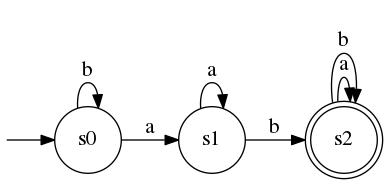
\includegraphics[scale=0.4]{./Img/automi/ex1.png}
\caption{Rappresentazione grafica di un DFA}
\label{fig:dfa}
\end{figure}

\end{ex}

\subsection{Linguaggio di un DFA}
Il linguaggio di un DFA è l'insieme di tutte le stringhe che il DFA accetta. 
Sia $a_1, a_2, \dots, a_n$ una sequenza di simboli. A partire dallo stato iniziale $s_0$, mediante la funzione di transizione $t$ si ha $s_1 = t(s_0, a_1)$ come stato raggiunto a fronte dell'ingresso $a_1$. Procedendo allo stesso modo per altri simboli, $s_i = t(s_{i-1}, a_i)$, si viene a creare una sequenza di stati raggiunti  $s_1, s_2, \dots, s_n$. La sequenza è accettata se e solo se si raggiunge uno stato finale $s_n \in F$.
\'E possibile introdurre il concetto di \emph{funzione di transizione estesa} che restituisce lo stato raggiunto quando a partire da uno stato si ha una sequenza di simboli d'ingresso, invece che un simbolo soltanto. La funzione di transizione estesa $\hat t: S \times \Sigma^* \mapsto S$ è definita come:
$$
\hat t(s, \underline \omega) = \begin{cases}
s & \underline \omega = \epsilon,\\
t(\hat t(q, \underline x), a) & \underline \omega = \underline x\,a
\end{cases}
$$

Dunque una stringa $\underline \omega = a_1\, a_2\,\dots\,a_n$ appartiene al linguaggio definito dall'automa se e solo se $\hat t(s_0, \underline \omega) \in F$.
Di conseguenza si definisce linguaggio del DFA $D = (S,\Sigma, t, s_0, F)$:
$$
L(D) = \{\,\underline \omega\,\,|\,\,\hat t(s_0, \underline \omega) \in F\,\}.
$$

\newpage
\section{NFA}
Un automa a stati finiti non deterministico (NFA: nondeterministic finite automaton) è una quintupla:
\begin{center}
	$N = (\Sigma,S,t,s_0,F)$
\end{center}
dove:
\begin{itemize}
\item $\Sigma$ è un alfabeto, ovvero l'insieme dei simboli di input;
\item $S$ è un insieme finito di stati;
\item $t$ è la funzione di transizione (non deterministica) $t: S \times (\Sigma \cup \{\epsilon\}) \rightarrow 2^S$ che associa, ad uno stato e un simbolo di input (oppure al simbolo vuoto $\epsilon$), un insieme di stati;
\item $s_0$ è lo stato iniziale;
\item $F \subseteq S$ è un insieme di stati finali.
\end{itemize}
La differenza tra gli automi deterministici e quelli non deterministici riguarda la funzione di transizione, che in quest'ultima classe di automi presenta due forme di non determinismo: da un lato, la presenza di $\epsilon$-transizioni può causare il cambiamento di stato dell'automa senza che venga consumato alcun simbolo in input; d'altro canto, la possibile presenza di transizioni uscenti dal medesimo stato con la stessa label fornisce una scelta non deterministica nella simulazione dell'automa.
Il teorema che è analizzato nella sezione successiva mostra che è sempre possibile, partendo da un NFA, ricostruire un corrispondente DFA equivalente.
L'utilizzo di automi non deterministici è dettato dalla maggior facilità di modellazione nell'ambito di alcuni algoritmi specifici, nonché da procedure note che permettono di costruire un automa non deterministico equivalente ad una espressione regolare data \footnote{Si noti che, come illustrato in \cite{book:compilers}, è altresì possibile partendo da un'espressione regolare costruire direttamente un DFA.}.\\
Le possibili rappresentazioni di NFA sono simili a quelle viste per i DFA, con piccole variazioni: nella rappresentazione tabellare ogni cella, invece che contenere un singolo stato, racchiude un insieme di stati, e come simboli si aggiunge una colonna che esplicita le transizioni scatenate dal simbolo vuoto; nella rappresentazione grafica, si ricorre a frecce con la label $\epsilon$ per indicare le $\epsilon$-transizioni.

\begin{ex}
Viene di seguito riportato un esempio di NFA.

\begin{table}[htbp]
\begin{center}
\begin{tabular}{r | c  c  c}
& a & b & $\epsilon$ \\ \hline
$\rightarrow s_0$ & $\emptyset$ & $\{s_4\}$ & $\{s_1,s_2,s_3\}$\\
$s_1$ & $\{s_4\}$ & $\emptyset$ & $\{s_3\}$\\
$s_2$ & $\emptyset$ & $\{s_3\}$ & $\emptyset$\\ 
$*s_3$ & $\emptyset$ & $\{s_4\}$ & $\emptyset$\\ 
$*s_4$ & $\{s_3\}$ & $\emptyset$ & $\emptyset$\\
\end{tabular}
\caption{Rappresentazione tramite tabella di un NFA}
\label{tab:nfa}
\end{center}
\end{table}

\begin{figure}[htbp]
\centering
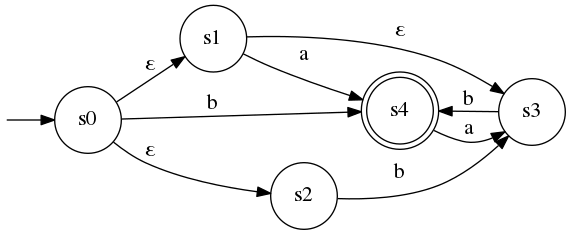
\includegraphics[scale=0.4]{./Img/automi/nfa.png}
\caption{Rappresentazione grafica di un NFA}
\label{fig:nfa}
\end{figure}

\end{ex}

\subsection{\texorpdfstring{$\epsilon$}-closure}
La $\epsilon$-closure di uno stato $s$ è l'insieme degli stati raggiunti a partire da $s$ tramite transizioni di stato senza simboli di input, ovvero mediante $\epsilon$-transizioni.
Formalmente $\epsilon\textit{-closure} : S \mapsto 2^S$ tale che:
$$
\epsilon\textit{-closure}(s) = \begin{cases}
\{s\} & t(s, \varepsilon) = \emptyset \\
\{s\} \cup \displaystyle \bigcup_{s_i \in A} \epsilon\textit{-closure}(s_i) & A = t(s, \varepsilon) \ne \emptyset
\end{cases}
$$
\'E inoltre possibile introdurre la nozione di $\epsilon$-closure per insiemi di stati, $\epsilon\textit{-closure}^*: 2^S \mapsto 2^S$:
$$
\epsilon\textit{-closure}^*(\mathbb{T} \subseteq S) = \displaystyle\bigcup_{s_i \in \mathbb{T}} \epsilon\textit{-closure}(s_i)
$$

\subsection{Linguaggio di un NFA}
Attraverso il concetto di $\epsilon$-closure è possibile definire in modo conciso la \emph{funzione di transizione estesa} per stringhe non contenenti il simbolo $\varepsilon$. 
Si definisce $\hat t:  S \times \Sigma^* \mapsto 2^S$:
$$
\hat t(s, \underline \omega) = \begin{cases}
\mathcal{E}\textit{-closure}(s) & \omega = \epsilon \\
\mathcal{E}\textit{-closure}^*(A) & \omega = \underline x \, a \,,\, A=\displaystyle\bigcup_{s_i \in B} t(s_i, a)\,,\,B=\hat t(s, \underline x)
\end{cases}
$$

Dunque una stringa $\underline \omega = a_1\, a_2\,\dots\,a_n$ appartiene al linguaggio definito dall'automa se e solo se $\hat t(s_0, \underline \omega) \in F$.

Di conseguenza si definisce linguaggio del NFA $N = (S,\Sigma, t, s_0, F)$:
$$
L(N_\varepsilon) = \{\,\underline \omega\,\,|\,\,\hat t(s_0, \underline \omega) \cap F \ne \emptyset\,\}.
$$


\newpage
\section{Subset construction}
A causa del loro non determinismo, spesso i NFA necessitano di essere convertiti in DFA per essere utilizzati e simulati in modo più intuitivo. La tecnica nota in letteratura per ottenere questa conversione è chiamata \emph{subset construction}.
L'idea generale di questo algoritmo è che ad ogni stato del risultante DFA corrisponde un insieme di stati del NFA di partenza.
Il primo problema che bisogna affrontare è quello di gestire le $\epsilon$-transizioni. Queste particolari transizioni indicano in quali stati l'automa può trovarsi contemporaneamente. L'operazione di $\epsilon$-closure permette di trovare, a partire da un particolare stato, tutti gli stati raggiungibili senza la consumazione di simboli in ingresso. Il primo passo della subset construction, quindi, consiste nell'assegnare allo stato iniziale del DFA risultante la $\epsilon$-closure dello stato iniziale del NFA in esame. L'algoritmo prosegue calcolando, per ogni possibile input ricevuto a partire da ogni stato del NFA contenuto nello  stato attuale del DFA, l'insieme degli stati raggiungibili, su cui viene effettuata la $\epsilon$-closure. Il procedimento procede in questo modo sino a che tutti i nuovi stati generati nel DFA non sono stati processati. Lo pseudocodice è fornito nell'algoritmo \ref{alg:subset}.
\'E possibile, teoricamente, che il numero di stati del DFA sia esponenziale nel numero di stati del NFA: tale numero è limitato superiormente dalla cardinalità dell'insieme potenza degli stati dell'automa non deterministico, cioè dal numero di tutti i possibili sottoinsiemi degli stati.
Fortunatamente questo caso pessimo raramente si presenta e per linguaggi reali spesso il numero di stati dei due automi è simile e il comportamento esponenziale non sussiste.

\begin{algorithm}
\textbf{SubsetConstruction($N$)}
\begin{algorithmic}
\STATE Sia $s_0$ lo stato iniziale del NFA, $Dstates$ gli stati del DFA risultante, $t$ la funzione di transizione del DFA
\WHILE{$\exists s \in Dstates$ non marcato}
	\STATE marcare $s$
	\FORALL{simbolo di input $a$}
		\STATE $U = \epsilon-closure(move(T,a))$
		\IF{$U \notin Dstates$}
			\STATE aggiungi $U$ come stato non marcato in $Dstates$
		\ENDIF
		\STATE $t(T,a) = U$
	\ENDFOR
\ENDWHILE
\end{algorithmic}
\caption{Algoritmo subset construction}
\label{alg:subset}
\end{algorithm}

\newpage
\section{Linguaggi}
Un automa a stati finiti possiede delle transizioni i cui simboli costituiscono l'alfabeto di un linguaggio e una stringa ottenuta percorrendo un cammino dallo stato iniziale ad uno stato finale si dice che appartiene al linguaggio. Una stringa caratterizzata da nessun simbolo dell'alfabeto è detta stringa vuota e si denota con $\epsilon$.
Data una stringa $s$, la sua lunghezza $|s|$ è il numero di simboli contenuti in essa, tenendo conto di eventuali occorrenze multiple del medesimo simbolo. Per convenzione, la lunghezza della stringa vuota è zero.
\begin{defn}
Un linguaggio definito su un insieme alfabeto $\Sigma$ è un insieme di stringhe di lunghezza finita formate da simboli appartenenti a $\Sigma$.
\end{defn}
L'operazione fondamentale per la costruzione di linguaggi è quella della concatenazione. Se $x$ e $y$ sono stringhe, la loro concatenazione è la stringa $xy$. La stringa vuota è l'elemento identità di tale operazione, poiché per ogni stringa $s$, $s\epsilon = \epsilon s = s$.\\
Un'altra operazione che caratterizza i linguaggi è la chiusura di Kleene, denotata $L^*$, che è l'insieme di tutte le stringhe finite che si ottengono concatenando elementi dell'alfabeto, compresa la stringa vuota.\\
Sui linguaggi è altresì possibile applicare tutte le operazioni insiemistiche quali l'unione, l'intersezione, la differenza e il complemento.
Un linguaggio può essere visto come un modo formale di descrivere il comportamento di un sistema, specificando tutte le possibili sequenze di eventi che esso è in grado di generare. 
Un automa è un formalismo in grado di rappresentare un linguaggio.
In particolare, nel seguito della trattazione, ci si focalizzerà sui cosiddetti linguaggi regolari, ovvero su quei linguaggi che possono essere rappresentati tramite automi con un numero finito di stati.

\section{Espressioni regolari}
Le espressioni regolari costituiscono quell'insieme di linguaggi che possono essere rappresentati da automi a stati finiti (grammatica di tipo 3 della gerarchia di Chomsky). Le espressioni regolari descrivono tutti i linguaggi costruiti applicando ai simboli appartenenti ad un alfabeto $\Sigma$ gli operatori di unione, concatenazione e chiusura. Le espressioni regolari sono generate ricorsivamente dalle sottoespressioni che le formano, secondo le seguenti regole.
\begin{enumerate}
\item $\epsilon$ è una espressione regolare che denota il linguaggio $L(\epsilon) = \{\epsilon\}$, 					contenente la sola stringa vuota;
\item se $a$  è un simbolo in $\Sigma$, allora $a$ è un'espressione regolare che denota il linguaggio $L(a) = 	\{a\}$, contenente la sola stringa di lunghezza unitaria $a$.
\item se $x$ e $y$ sono espressioni regolari che denotano rispettivamente i linguaggi $L(x)$ e $L(y)$, allora:
	\begin{itemize}
	\item $(x)$ è l'espressione regolare che denota il linguaggio $L(x)$;
	\item $(x) | (y)$ è l'espressione regolare che denota il linguaggio $L(x) \cup L(y)$ (unione);
	\item $(x)(y)$ è l'espressione regolare che denota il linguaggio $L(x)L(y) = \{xy | x \in L(x), y \in L(y)\}$ (concatenazione);
	\item $(x)^*$ è l'espressione regolare che denota il linguaggio $(L(x))^*$: ripetizione zero o più volte di stringhe in $L(x)$ (chiusura di Kleene).
	\end{itemize}
\end{enumerate}
Altri operatori possono essere definiti opportunamente in base al dominio applicativo, generando espressioni regolari estese.

\subsection{Costruzione di Thompson}
La costruzione di \emph{McNaughton- Yamada- Thompson}(o semplicemente costruzione di Thompson) è in grado di convertire una espressione regolare in un NFA caratterizzato dal medesimo linguaggio. L'algoritmo opera scomponendo l'espressione regolare in un albero sintattico e costruendo un NFA per ogni sottoespressione, in maniera bottom-up, utilizzando le $\epsilon$-transizioni come "collante" per unire i sottoautomi. L'automa risultante permette di riconoscere se una stringa appartiene o meno al linguaggio relativo all'espressione regolare di partenza.\\
La regola base del metodo, rappresentata in figura \ref{fig:re_atom}, genera un NFA da una sottoespressione atomica, composta da un solo simbolo $a$ o dal simbolo nullo $\epsilon$. L'automa generato è composto da due stati, uno iniziale e l'altro finale, e una transizione in corrispondenza del simbolo atomico dallo stato iniziale allo stato finale.
Le regole induttive permettono di ricavare ricorsivamente l'intero automa.
Si supponga che $N(s)$ e $N(t)$ siano gli NFA ricavati dalle espressioni regolari $s$ e $t$ rispettivamente.
\begin{enumerate}
\item Si supponga $r = s|t$. L'automa $N(r)$ equivalente all'espressione regolare $r$ è costruito in figura \ref{fig:re_union}. Sono creati due nuovi stati, uno iniziale e uno finale. Due $\epsilon$-transizioni uniscono lo stato iniziale del nuovo automa agli stati iniziali di $N(r)$ e $N(s)$. Si noti che gli stati finali di $N(r)$ e $N(s)$ non sono finali nel nuovo automa, e una $\epsilon$-transizione collega ciascuno al nuovo stato finale. Il linguaggio dell'automa generato è l'unione dei linguaggi dei due automi di partenza.
\item Si supponga $r = st$. L'automa $N(r)$ equivalente all'espressione regolare $r$ è costruito in figura \ref{fig:re_concat}. Lo stato iniziale di $N(s)$ diviene in nuovo stato iniziale di $N(r)$, mentre lo stato finale di $N(t)$ costituisce il nuovo stato finale dell'automa risultante $N(r)$ . Il linguaggio dell'automa generato è la concatenazione dei linguaggi dei due automi di partenza.
\item Si supponga $r = s^*$. L'automa $N(r)$ equivalente all'espressione regolare $r$ è costruito in figura \ref{fig:re_closure}. Sono creati due nuovi stati, uno iniziale e uno finale. A partire dallo stato iniziale, vengono poste due $\epsilon$-transizioni: una verso lo stato iniziale di $N(s)$, l'altra verso il nuovo stato finale. Inoltre è aggiunta una $\epsilon$-transizione dallo stato finale per $N(s)$ al suo stato iniziale per $N(s)$. Il linguaggio dell'automa generato dalla chiusura di Kleene dei linguaggi dei due automi di partenza.
\item Si supponga $r = (s)$. Allora il linguaggio di $r$ coincide con quello di $s$, e come automa $N(r)$ può essere utilizzato l'automa di partenza $N(s)$.
\end{enumerate} 


\begin{figure}[htbp]
\centering
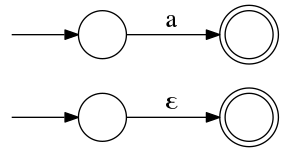
\includegraphics[scale=0.4]{./Img/automi/re_atom.png}
\caption{NFA per espressioni regolari atomiche}
\label{fig:re_atom}
\end{figure}


\begin{figure}[htbp]
\centering
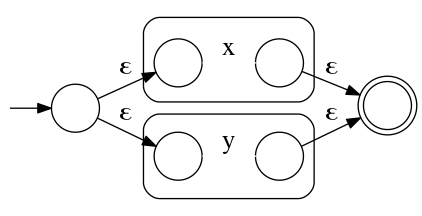
\includegraphics[scale=0.4]{./Img/automi/re_union.png}
\caption{NFA per l'unione di due espressioni regolari}
\label{fig:re_union}
\end{figure}

\begin{figure}[htbp]
\centering
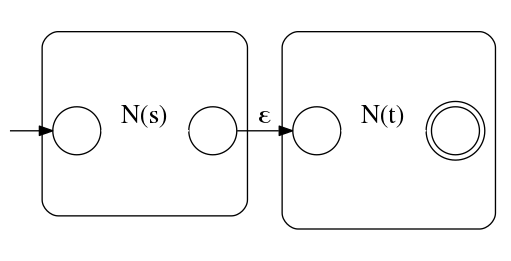
\includegraphics[scale=0.4]{./Img/automi/re_concat.png}
\caption{NFA per la concatenazione di due espressioni regolari}
\label{fig:re_concat}
\end{figure}

\begin{figure}[htbp]
\centering
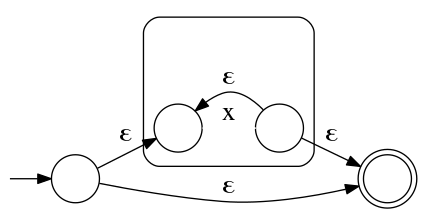
\includegraphics[scale=0.4]{./Img/automi/re_closure.png}
\caption{NFA per la chiusura di un'espressione regolare}
\label{fig:re_closure}
\end{figure}


\newpage
\section{Minimizzazione degli stati}
Dato un linguaggio, possono esistere più automi deterministici che lo riconoscono. Si cerca sempre di scegliere l'automa che presenta il minor numero di stati, dato che l'implementazione di quest'ultimo consente di risparmiare memoria e tempo nella simulazione. 
Esiste sempre un unico DFA minimo per ogni linguaggio regolare, a meno di una ridenominazione del nome degli stati. Questo particolare automa può essere costruito raggruppando insieme quegli stati che sono tra loro equivalenti. Per capire come verificare tale equivalenza, si ricorre al concetto di distinguibilità.
\begin{defn}
La stringa $x$ distingue lo stato $s$ dallo stato $t$ se esattamente uno degli stati raggiunti partendo da $s$ e da $t$ seguendo il cammino con label $x$ è uno stato finale. Quindi, lo stato $s$ è distinguibile dallo stato $t$ se esiste una stringa che li distingue.
In particolare, la stringa vuota distingue ogni stato finale da qualsiasi stato non finale.
\end{defn}

L'algoritmo di minimizzazione degli stati funziona partizionando gli stati dell'automa in gruppi di stati indistinguibili. 
In ogni istante, l'algoritmo mantiene partizioni di stati che non sono ancora stati distinti.
Inizialmente gli stati sono divisi in due macro-partizioni, una contenente gli stati non finali, l'altra contente quelli finali. La divisione iniziale viene raffinata individuando un simbolo di input che distingue tra loro alcuni degli stati appartenenti ad un gruppo, generando in questo modo una ulteriore suddivisione interna. La procedura viene applicata fino a quando nessun gruppo, per ogni simbolo di input, può essere scisso nuovamente.
Infine ogni gruppo di stati, scegliendo per ogni insieme uno stato come rappresentante, viene fuso in un singolo stato che appartiene all'automa minimo risultante. 